\documentclass[11pt, oneside]{article}   	% use "amsart" instead of "article" for AMSLaTeX format
\usepackage{geometry}                		% See geometry.pdf to learn the layout options. There are lots.
\geometry{letterpaper}                   		% ... or a4paper or a5paper or ... 
%\geometry{landscape}                		% Activate for for rotated page geometry
%\usepackage[parfill]{parskip}    		% Activate to begin paragraphs with an empty line rather than an indent
\usepackage{graphicx}				% Use pdf, png, jpg, or eps� with pdflatex; use eps in DVI mode
								% TeX will automatically convert eps --> pdf in pdflatex		
\usepackage{amssymb}
\usepackage{amsmath}
\usepackage{parskip}
\usepackage{color}
\usepackage{hyperref}

\title{Green's Theorem for complex variables}
%\author{The Author}
%\section{}
%\subsection*{}
\date{}							% Activate to display a given date or no date

\graphicspath{{/Users/telliott_admin/Dropbox/Tex/png/}}
% \begin{center} 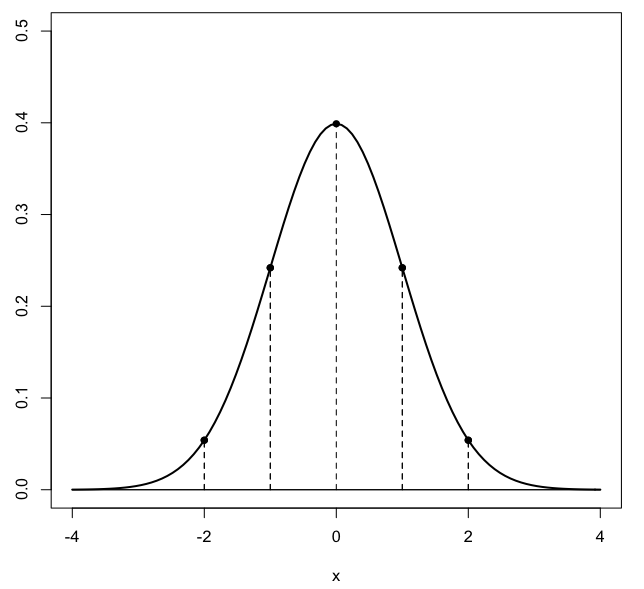
\includegraphics [scale=0.4] {gauss3.png} \end{center}
\begin{document}
\maketitle
\Large
We can state Green's Theorem for complex variables as
\[ \oint f(z) \ dz = i \iint \frac{\partial f}{\partial x} + i  \frac{\partial f}{\partial y}  \ dx \ dy \]
As an example, consider the curve going around the square $[-1,-i] \times [1, i]$ and the function $f(z) = |z|^2$.  So
\[ f(z) = |z|^2 = zz* \]
\[ = (x + iy)(x - iy) \]
\[ = x^2 + y^2 \]
Then 
\[ f_x = 2x, \ \ \ f_y = 2y \]
and
\[ I = \iint 2x + i 2y \ dx \ dy \]
The inner integral is
\[ \int_{-1}^1 2x + i 2y \ dx = 2x^2 + i 2xy \ \bigg |_{-1}^1 = 4iy \]
The outer integral is
\[ I = \int_{-1}^1 4iy \ dy = 2i y^2 \ \bigg |_{-1}^1 = 0 \]
\subsection*{$C_1$ + $C_3$}
\[ I = \int u \  dx - \int v \ dy + i \ [ \ \int u \ dy + \int v \ dx \ ] \]
Along $C_1$, $dy = 0$ and so the line integral is
\[ I = \int u \  dx + i \int v \ dx \]
The function is $u(x,y) = x^2 + y^2$, $v(x,y) = 0$ so
\[ I = \int x^2 + y^2 \  dx \]
With $y=1$ this is
\[ I = \int_1^{-1} x^2 + 1 \  dx = \frac{x^3}{3} + x \ \bigg |_1^{-1} \]
\[ = (-\frac{1}{3} - 1) - (\frac{1}{3} + 1) = -\frac{8}{3} \]
Along $C_3$, with $y = -1$ (and $y^2 = 1$) this is
\[ I = \int_{-1}^{1} x^2 + 1 \  dx = \frac{x^3}{3} + x \ \bigg |_{-1}^{1} \]
\[ = (\frac{1}{3} + 1) - (-\frac{1}{3} - 1) = \frac{8}{3} \]
so these two line integrals cancel.

\subsection*{$C_2$ + $C_4$}
\[ I = \int u \  dx - \int v \ dy + i \ [ \ \int u \ dy + \int v \ dx \]
Along $C_2$ and $C_4$, $dx = 0$ and so the line integral is
\[ I = - \int v \ dy + i \ \int u \ dy \]
The function is $u(x,y) = x^2 + y^2$, $v(x,y) = 0$ so
\[ I =  i \ \int x^2 + y^2 \ dy \]
With $x = -1$ or on $C_4$, $x = 1$, in either case $x^2 = 1$ so we have the same integral along opposite paths, (multiplied by $i$), so we have the same answer for the two together:  $0$.





\end{document}  